\chapter {Иорданский ручей}

Об Иорданском ручье сведения неясны. 

На нескольких картах стыка 19 и 20 веков отмечен, однако не подписан, ручей, берущий начало в глубине существовавшего тогда оврага по Мыльному переулку, и продолжающийся на северо-восток в сторону Чернечьего («старого» Иорданского) озера, подробнее о котором сказано в главе про Почайну.

Киевские диггеры называют Иорданским ручей, что начинается приблизительно от источника на территории новой, построенной в котловине бывшего глиняного карьера, Никольско-Иорданской церкви, затем текущий в трубе под Мыльным переулком и далее под улицей Заводской в сторону Гавани, очень вероятно повторяя путь ручья, упомянутого абзацем выше.

Я хочу разобраться, что называли Иорданским ручьем в 19 веке. Разобраться трудно, ибо прошло много времени и местность сильно изменилось. Как вообще работает родник в склоне горы, или, говоря языком геологии, пластовый источник? 

Гора состоит из слоев грунта. Осадки впитываются в эти слои до некоего нижнего слоя, который не пропускает воду. Это может быть, например, слой глины, которая, намокая, перестает проводить воду. Слои, копящие в себе воду, называются водоносным горизонтом. Если водонепроницаемый слой имеет уклон в сторону склона, то вода из горизонта начинает туда двигаться и выходить на поверхность в виде родника.

Водонепроницаемый слой может быть на уровне середины горы, или внизу – как получится. А чем больше площадь водоносного горизонта и его толщина, тем больше он может впитать воды и снабжать ею источник, если, конечно, сам горизонт в свою очередь получает питание от осадков.

Склоны же Лысой горы и окрестностей столь великое множество раз перекапывались и уничтожались, что водоносный горизонт и водонепроницаемый слой многократно изменялись. Значит, выходы родников из склона могли смещаться, и сейчас пожалуй нельзя восстановить историю здешней природной водной системы.
 
Как мы знаем, где-то около Иорданской церкви было нечто вроде колодца, куда поступала вода по трубам из другого колодца, наверху горы. Этот нижний колодец и слыл чудодейственным Иорданским источником. Поскольку современная Иорданская церковь находится на другом месте, чем прежняя, то современный источник, откуда берут воду прихожане – вероятно тоже в другом месте.

Возникает несколько вопросов относительно положения дел в 19 веке. Имеет ли отношение ручей, протекавший в Мыльном переулке, к источнику?

Вспомним сообщение Лохвицкого: 

\begin{quotation}
Ручей Иорданский пониже и подле сего места течет, а вытекает повыше, с горы, близ сих остатков Ильинской церкви. Сей ручей начало берет из ключей железистых, которые приметны по ржавчине железной в источнике родника сих ключей.
\end{quotation}

Вот бы знать еще точно, где сии «остатки» были... Но явно на холме у задворков нынешних фабрик молочной кислоты и нотной. Что там сейчас?

По нижней половине склона от Богуславского спуска до Иорданского переулка (на картах его любят обозначать тоже Мыльным), под горой с дачами «Кожевника», не достигая долготы нотной фабрики, есть дренажная система, местами доступная для просмотра. В бетонных комнатках видны толстые керамические трубы и течение воды. Уже над фабрикой молочной кислоты, в одном из открытых узлов системы просматривается труба откуда-то сверху, со стороны «древней дороги на Лукьяновку». В зарослях ближе к оврагу с этой дорогой, прямо из горы сочится бурый родник, увлажняя смешанную с грязью траву и листья.

Лохвицкий говорил что ручей Иорданский составлялся из нескольких, именно нескольких «ключей железистых». Родники, сливаясь, и давали более ощутимый, чем по отдельности, поток.

Вот несколько снимков 2013 года с задворков фабрики молочной кислоты.

Сначала – колодец захвата грунтовых вод, оттуда труба ведет примерно на, как я помню, юго-восток:

\begin{center}
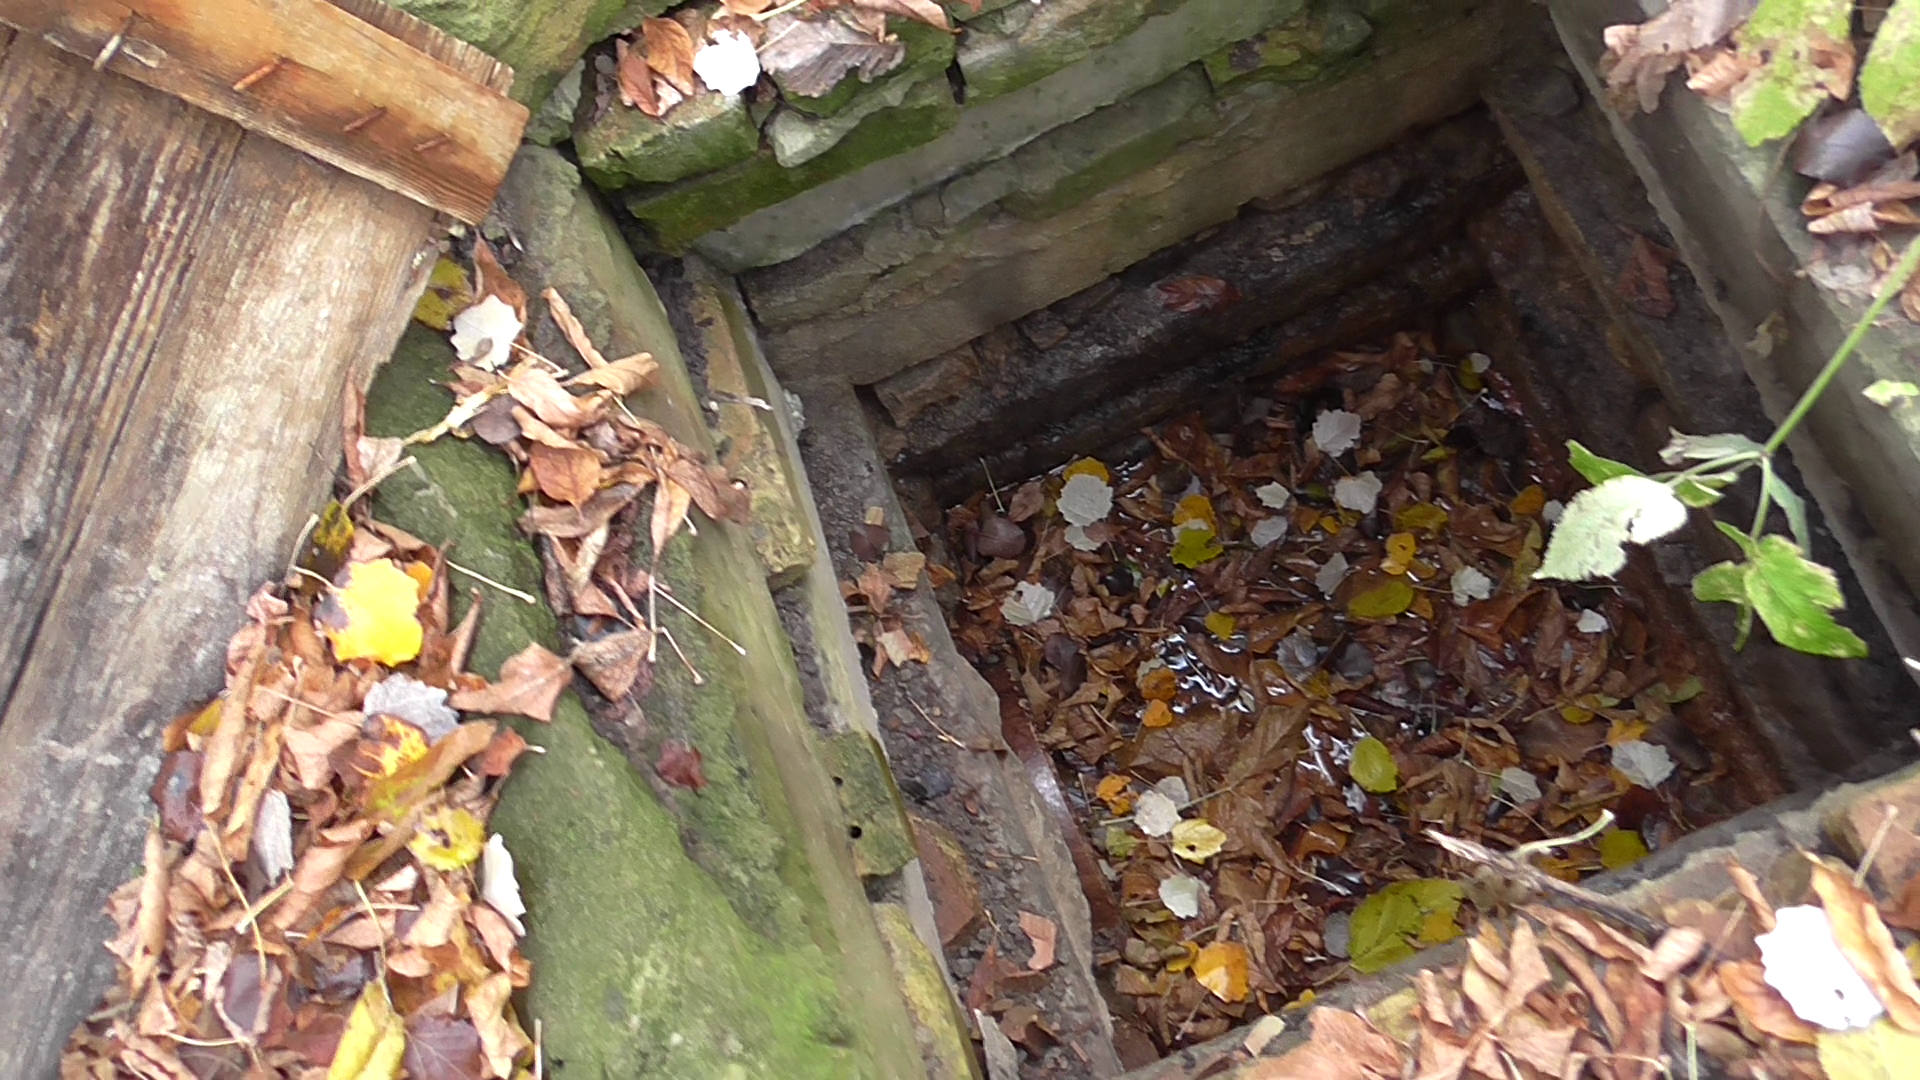
\includegraphics[width=\linewidth]{chast-kirvys/iordanruch/s_vlcsnap-2014-05-16-20h08m14s138.jpg}
\end{center}

А вот место, где собирается вода из двух труб и направляется в трубу на северо-восток, в направлении фабрики молочной кислоты и улицы Кирилловской. Рыжее на снимке и есть признак «железистости». Её можно наблюдать на родниках из склонов озера Глинки, а также в ручьях Репяхового и Бабьего яров.

\begin{center}
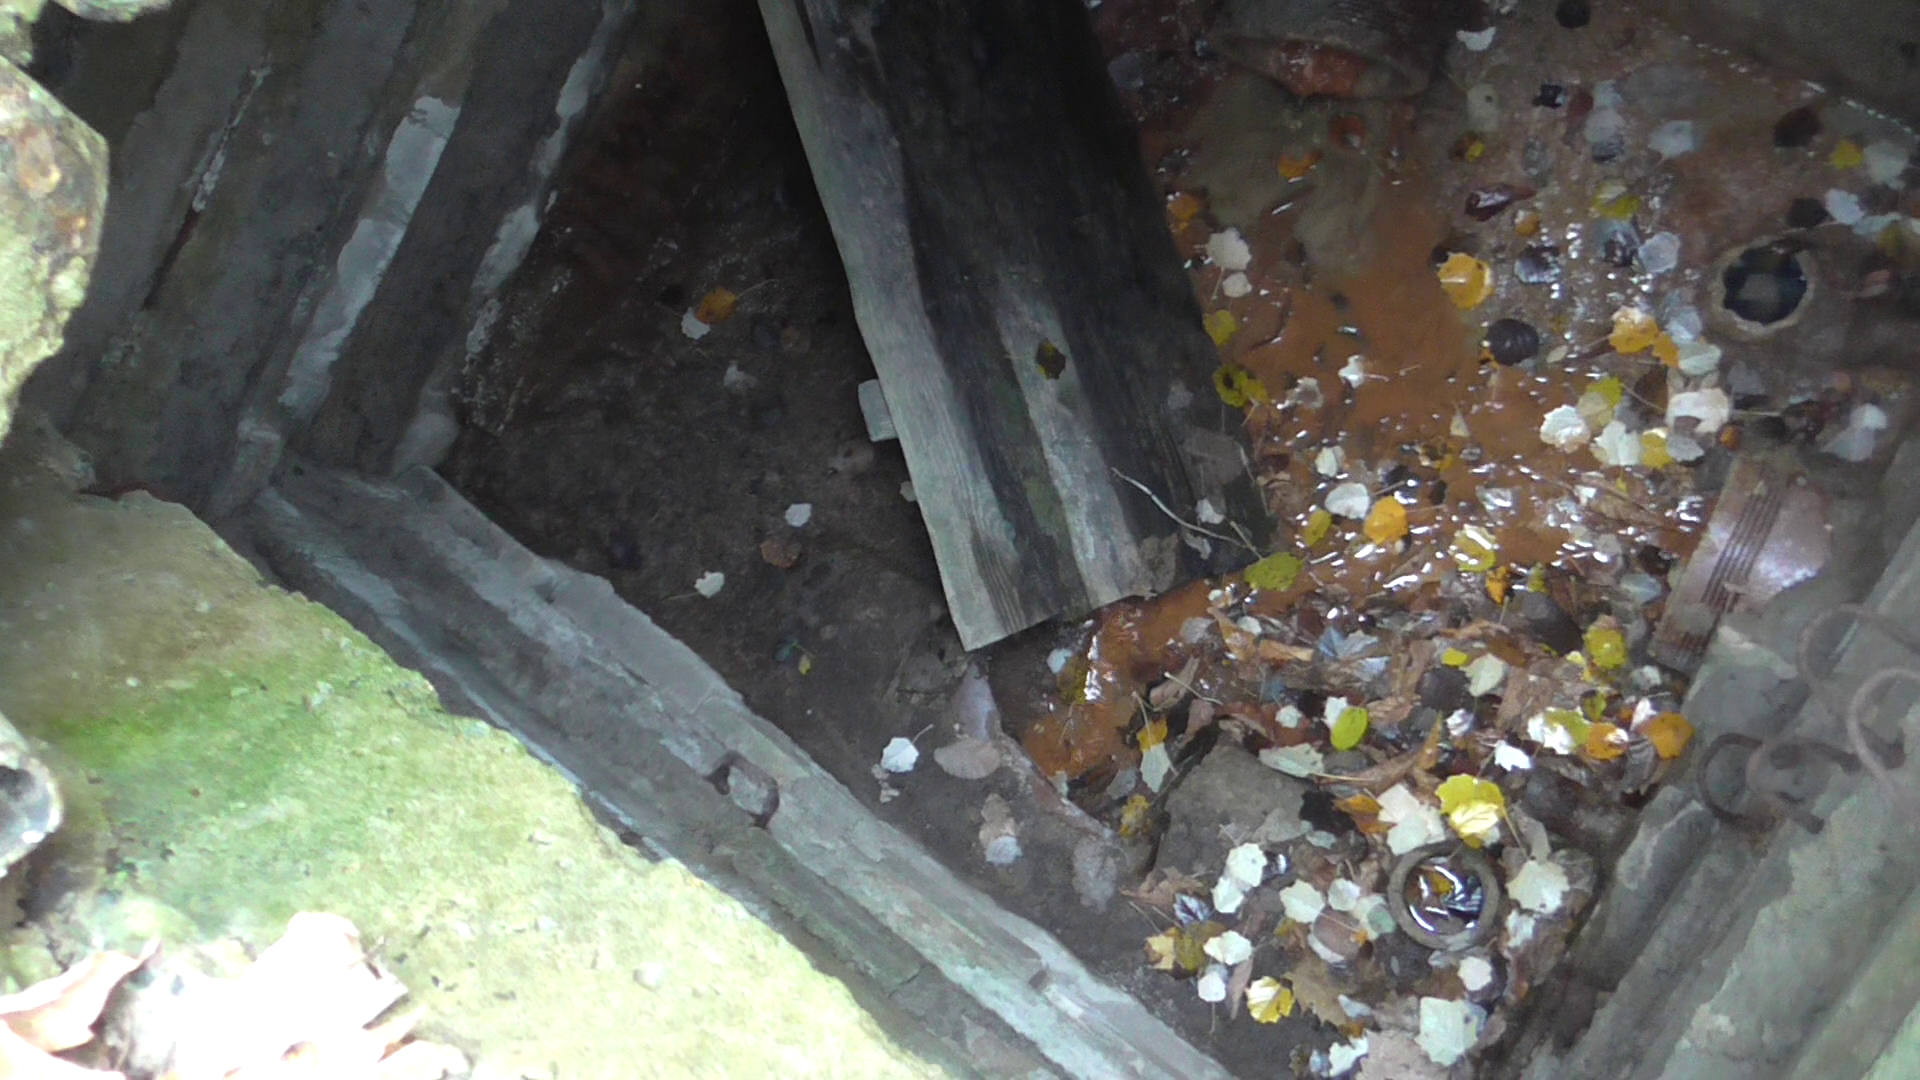
\includegraphics[width=\linewidth]{chast-kirvys/iordanruch/s_vlcsnap-2014-05-16-20h10m19s241.jpg}
\end{center}

Что же, Иорданский ручей начинался над нынешней фабрикой молочной кислоты? Куда он тёк дальше?

Меня беспокоит ручей по Мыльному переулку на картах. От задворков фабрики молочной кислоты ручей туда бы не стекал. Его естественный ход – в сторону улицы Кирилловской. Поэтому я не знаю, какое отношение имеет ручей в переулке к тому, описанному Лохвицким, Иорданскому ручью, что рождался на горе примерно в районе «усадьбы Марр» и над Иорданской церковью. 

Может, в старину, с горних тылов фабрики молочной кислоты воду ручья именно трубами направляли куда-то еще.

Но вспомним сообщение Похилевича о «монастырском колодце, существующем и ныне на уступе горы, выше нынешнего церковного погоста, из которого проведена трубами превосходная вода в нижний, близ нынешней церкви».

Это значит, что вода в нижний колодец была проведена из верхнего на уступе горы, выше кладбища. А описанная мною дренажная система – на одной с ним высоте, у самого основания кладбища.

Какой уступ имеет в виду Похилевич? В какую сторону от старинного подъема на Лукьяновку, то бишь над юго-восточной или северо-западной частью кладбища? Если первое, то источник ближе к Лысой горе, если второе – то к мысу с дачами «Кожевника». В любом случае, речь идет о склонах усадьбы Марр и над бывшей Иорданской церковью.

Верхнего же колодца – еще выше «кладбищенской» дренажки – я на склонах не видел. И немудрено, ибо с того времени, как его описал Похилевич, прошло много лет, а местность многократно перекраивалась.

Учитывая большую даже сейчас насыщенность там водоносного горизонта и множество родников, полагаю следующее. Иорданский ручей слагался из ручьев, текущих со северо-восточного склона Лысой горы и юго-восточного склона холма дач «Кожевника». Ручей был достаточно велик, чтобы Лохвицкий смог проследить его течение до устья в Иорданское озеро. 

Есть сведения, что Иорданский ручей протекал в сторону улицы Кирилловской между Иорданским и Богословским монастырями, разделяя их помимо рукотворной ограды. Около схода со склона к Иорданскому переулку, по заброшенной лестничке близ развалин старого дома есть остатки коллектора. 

Книга Похилевича издана в 1865 году. Сказано о двух колодцах, верхнем и нижнем, куда поступает вода из верхнего.

Может быть, привлечение еще одного источника, правда с разницей в 30 лет с книгой Похилевича, что-то прояснит?


И вдруг на плане 1837 года я нашел подробное изображение обоих ручьев!

\begin{center}
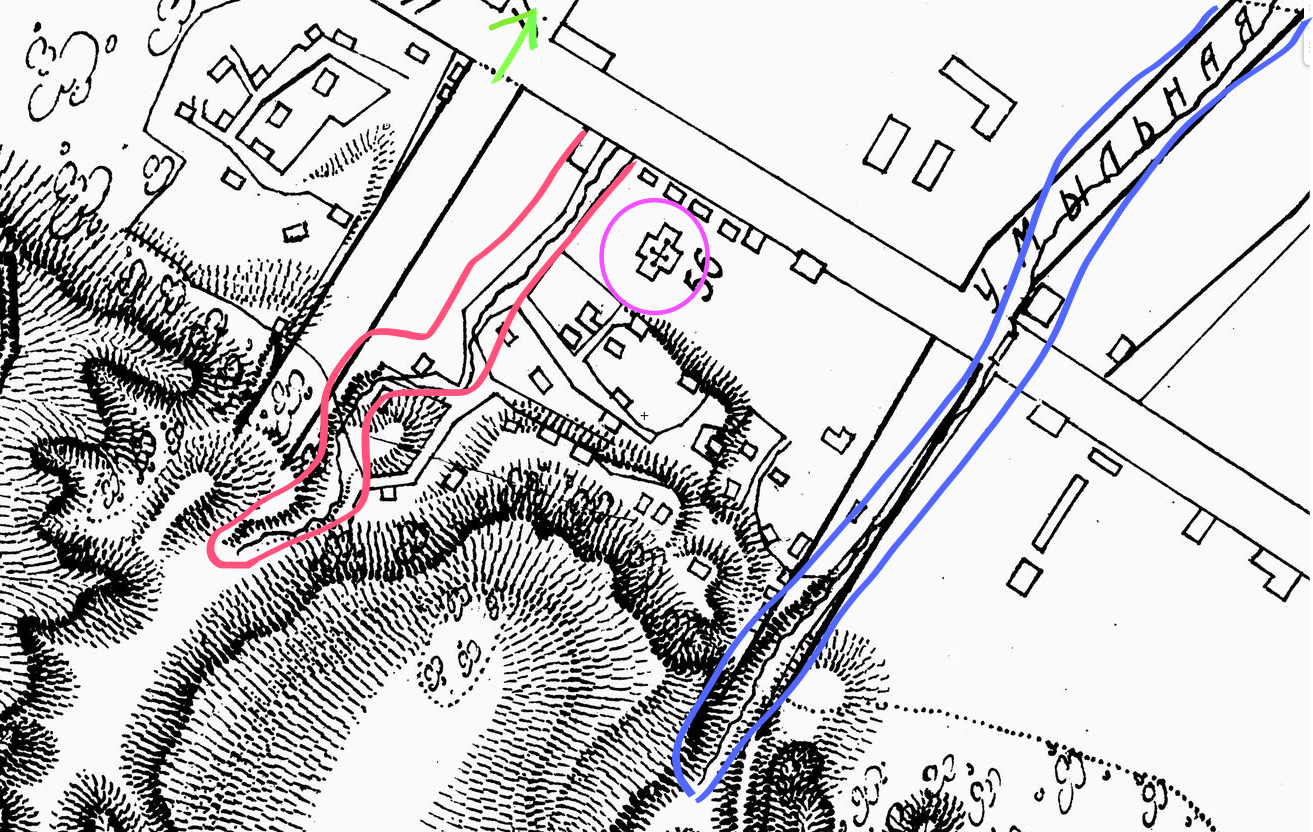
\includegraphics[width=\linewidth]{chast-kirvys/iordanruch/map.png}
\end{center}

Зеленая стрелочка - показана улица Заводская, она и ныне там. Мыльная улица исчезла, ею бы продолжался современный Мыльный переулок. Перпендикулярная улица, конечно же, Кириловская. Синим я отметил ручей, вытекающий - о да - из Мыльного переулка, и при наложении на спутник имеет устье этого ручья точнехонько в источнике близ современной Иорданской церкви-новодела. Этот источник сочится из подножия склона.

Фиолетовым я отметил прежнюю Иорданскую церковь.

Розовым - тот самый ручей, что берет начало на склоне выше старой Иорданской церкви. При наложении на спутник получаем, что он протекал... Вдоль "старого Никольского ввоза", дороги в овраге между мысом Лысой горы и "Кожевником"!

При этом, повторюсь, все задворки церкви (ныне задворки фабрики молочной кислоты), я обвел их желтым, это подножие холма - все они сочатся родниками, взятыми в дренажку, но прежде они тоже куда-то стекали.

Дальнейшее движение "розового" ручья на карте не показано. Однако именно он подходит под письменные описания Иорданского ручья - начинается на склоне над церковью, в самом деле разделял бы Иорданский и Богословский монастыри.


%В таком случае возвращаемся к вопросу о том, что за ручей вытекал из параллельного Мыльного переулка? Другой ручей? Или то был отвод от колодца, если нижний колодец находился именно в Мыльном переулке? За недостатком надежных данных решить эту задачу не могу.


Источник редкий, приведу его полностью. Это план Иорданского монастыря за 1835 год, со всеми его строениями. Легенду карты (с ошибками подлинника, но частичным приведением к современному написанию) даю текстом, а сам план – фотокопией.

План местоположению упраздненного Иорданского женского монастыря, снятому по Указу киевского губернаторского правления состоящему в ? части города Киева на Плоском, который назначен в обращение в приходскую церковь, с показанием на сем плане числа квадратных сажень исчисленных, по примерному назначению пространства для церковного погоста и в остающейся части занимаемой под заселение онаго монастыря, что означенно красными линиями, с объяснением кому именно находящиеся на нем деревянные кельи и строения ныне принадлежат.

ОБЪЯСНЕНИЕ ПЛАНА

А: Место примерно назначаемое для церковного погоста, Заключающее пространства тысячу шесть сот семдесят пять с одною третью квадратных сажень; на коем находятся деревянные строения именно:

1. Церковь во имя святителя и Чудотворца Николая.

2. Теплая церковь во имя святителя Димитрия Мироточца.

3. Колокольня. 

4. Корпус начальничьих келий и сараи.

5. Келья девицы Евдокии Бриенковой.

6. Монахини Надежды.

7. Монахини Евсесии.

8. Монахини Елены и вдовы дияконихи Марины Дьяковской.

9. Монахини Калиствены Степиодоты.

10. Монахини Порьфирии.

11. Манахини Евлампии.

12. Монахини Мокрины.

13. Вдовы священнической жены Евдокии.

14. Монахини Евгении.

15. Вдовы подпорутчицы Евдокиии Тюриковои и девицы Агафии Гриневичевой.

16. Монахини Спеклитикии.

17. Девицы Ефимии Димченковои.

18. Небольшой анбарчик вдов Ефросинии Дьяченковои и Устины Котлярки, и девицы Настасьи Шевченковои, коих келья за границею погоста.

19. Прежде бывшая келья монахинь Мамельхи и Серафимы, а ныне купленны Церьквою.

20. Монахини Палагеи.

21. Церковнои сараи.

22. Монахини Смарагды.

23. Вдовы священнической жены Ксении Бурмовской и монахини Нектарии.

24 Келья и сарай вдовы придворного Ганнимебера Феодосиии Петровой.

25. Колодец.

В: За исключением погоста остающаяся часть оного монастиря заключающая пространства три тысячи триста девятдесят и две три квадратных сажень, на которой находятся деревянные строения именно:

26. Келья и два сарая Скимонахини ксении.

27. Келья и погреб молдавской монахини Александры.

28. Молдавских монахинь Феофанны и Павлины.

29. Мещанки вдовы Елены Крамаренковой.

30. Девицы Акилины Петровой.

31. бывшая келья мещанки Анны Морозовой, а ныне мещанина Герасима Ермаченко.

32. Девицы Евдокии Герасимовой и вдовы Евдокии Корнилиевой.

33. Монахини Павлы.

34. Монахини Мокрыны.

35. Вдовы Ефросинии Дьяченковой и Устины Котлярки и Девицы Настасии Шевченковой.

36. Келья и сарай бывшие монахини Александры, а ныне вдовы Анны Морозовой.

37. Келья бывшая монахини Анфии а ныне мещанина Зеновия Савченка.

38. Келья, коморка и сараи бывшие монахинь Проклы и Палладии, а ныне мещанина Козьмы Шевченка.

39. Келья и сараи девицы Дарьи Буровой.

40. Бывшая монахини Марьяны, а ныне мещанки вдовы Евдокии Скляревской.

41. Келья и сараи Сержантши Домны Савельевой.

42. Солдатки вдовы Татьяны Фоминцовой.

43. Келья бывшая монахини Арсавии, а ныне пономаря Никиты Гилевича.

44. Мещанок вдов Ульяны Котляровой и Устины Михаревой.

45. Вдовы Губернской секретарши Евдокии Гриневской.

46. Две кельи девицы Прасковьи Синютиной.

47. Вдовы Ксении Штанькевички.

48. Бывшая келья монахини Евсевии а ныне а ныне мещанина Ивана Головаченка.

49. Солдата Яковлева.

50. Две кельи девицы Марфы Андреевой.

51. Вдовы Анны Марченковой.

52. Девицы Натальи Воиновой.

53. Вдовы Анны Садововны.

54. Вдовы солдатки Степаниды Лебедевой.

55. Девицы Меланьи Девятисиловны.

56. Девицы Ефимии Батяниной.

57. Девицы Настасии Дичинской.

58. Мещанки вдовы Аксиньи Корчинской.

59. Келья и анбар вдовы Кронтшадского Гезеля Ульяны Ушаковой.

60. Мещанки Екатерины.

61. Девицы Екатерины Жидовозновны.

62. Вдовы Козачки жены Екатерины Крымченковой.

63. Девиц Варвары и Ирины Лупичевских.

64. Девицы Агафии Степуровны.

65. Вдовы Евдокии Федоровой.

66. Девицы Харитины и вдовы Агафии Ромурки.

67. Девицы Домникии Ванфевны.

68. Вдовы Попадьи Анны.

69. Принадлежащая келья монахини Елены.

70. Вдовы салдатки Февроньи Шевелевой и вдовы мещанки Марины Лозовской.

71. Кладбище.

72. Два Колодца.

С. в оной остающейся части монастыря наложенной проекте вновь улицам с означением кварталов под желтою краскою, и что отходит под те улицы в сломку покрыто жидкою тушью.

\begin{center}
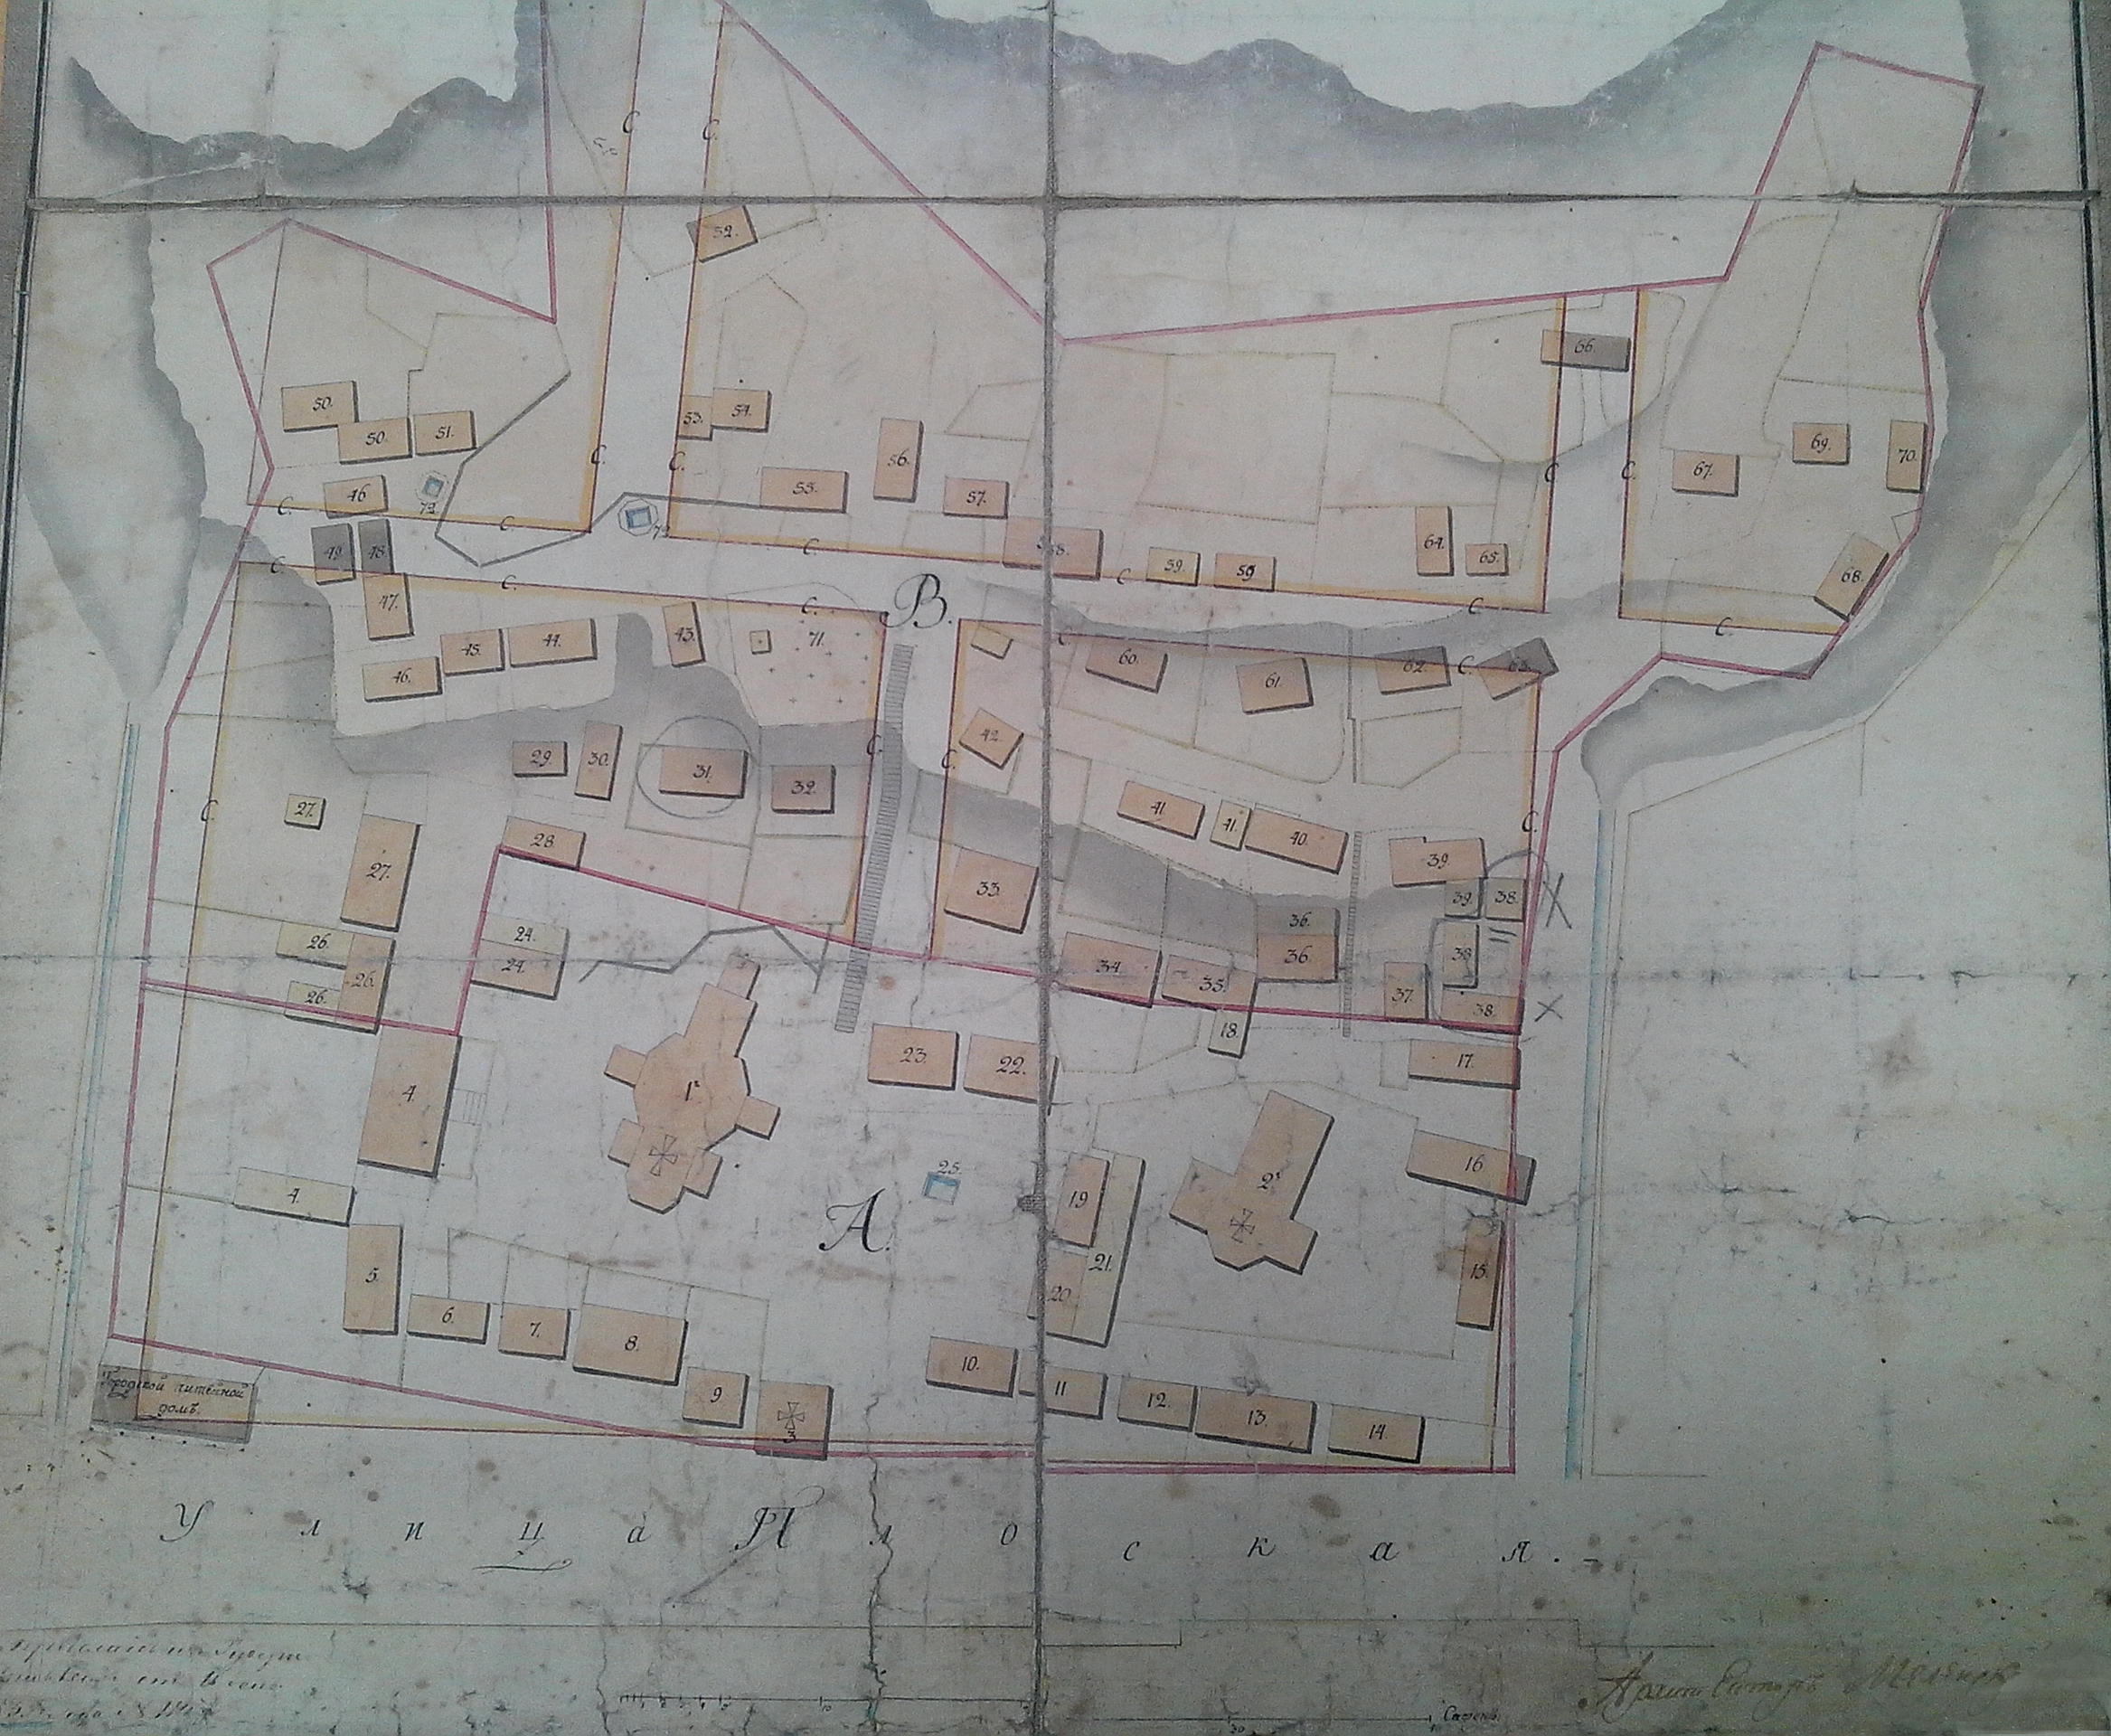
\includegraphics[width=\linewidth]{chast-kirvys/iordanruch/IMG_20170627_142118.jpg}
\end{center}

Карту нельзя однозначно наложить на современную, хотя соблазнительно ограничить изображенную усадьбу церкви переулком Мыльным с одной стороны, а Иорданским с другой, однако при пропорциональном уменьшении карты, для умещения на этом отрезке, кладбище получается под склоном горы, а не на оном. К сожалению, на карте нет внешних, вне пределов монастыря, ориентиров для привязки к местности.

Улица Кирилловская именована Плоской.

Большая Николаевская церковь обозначена номером 1. Ранее я приводил сведения, что она сгорела в 1821 году, но поскольку карта 1835-го – если я верно разобрал дату в нижнем левом ее углу – и церковь тут показана, значит сгорела не в 1821-м. Поодаль стоит деревянная Дмитриевская церковь, под номером 2, вместо которой потом построили где-то поблизости одноименную каменную. Я не могу соотнести места этих двух церквей с современным рельефом.

Голубые «каналы» по обеим сторонам усадьбы – не пущенные ли по канавам ручьи?

Кладбище, под номером 71 (слева от буквы «В») – сопоставимо ли с террасой, где поныне сохранился кусочек кладбища?

Буквой «А» помечено место, «назначаемое для церковного погоста». А Похилевич в 1865 году упомянул о:

\begin{quotation}
монастырском колодце, существующем и ныне на уступе горы, выше нынешнего церковного погоста, из которого проведена трубами превосходная вода в нижний, близ нынешней церкви.
\end{quotation}

На карте 1835 года мы видим рядом с буквой «А» колодец под номером 25, а выше (имею в виду не высоту над уровнем моря, но положение на карте) еще два колодца, слева от буквы «В». К букве же ведет лестница, и около «В» показано существующее в то время кладбище. Прикидывая к современному рельефу и учитывая положение келий – деревянных домиков – рядом с этим кладбищем, думаю, что оно всё же отлично от места сохранившегося поныне кусочка кладбища.

А может быть то изображена не лестница, но дорога между оврагами, «Никольский ввоз»?

Во всяком случае, карта дает понять, что склон горы над церковью был застроен домиками. Постепенно, к 20 веку, эти домики вытеснялись разрастающимся кладбищем. Сколь далеко наверх по склону простирались домики, на какой высоте они заканчивались – я не могу судить.


Доселе я не касался разбора названия Иорданского монастыря, приводя лишь расхожую легенду о чудесном источнике, где всплыл ковшик, уроненный паломником в палестинской реке Иордан. Кстати неясно, к какому времени относится возникновение предания. Замечу, я не подвергаю сомнению его истинность. Я верю в чудеса, верю, что ковшик мог быть обронен и затем появился за много километров. Но проверить нельзя. 

Однако, если предание возникло уже после того, как монастырь назвался Иорданским, значит оно – чистая выдумка для привлечения паломников. Церковь «святого Миколы Иорданского» в документах 17 века упоминается без каких-либо сведений о связанном с нею предании. И кстати, за три века – 17, 18, 19 – расположение колодцев могло меняться.

Но откроем словарь Даля.

\begin{quotation}
ИОРДАНЬ ж. место па льду и прорубь, для водоосвящения на Крещенье, [место, приспособленное для празднования освящения воды 6-го января]. Во иордани купаются, кто о святках  рядился. || Твр. прорубь вообще; котловинка, род колодца у болота, откуда течет ручей.
\end{quotation}

Была грязь, болото около монастыря? Была. Даже на плане Ушакова 1691 года отмечены «мостки на грязи». А колодец, откуда течет ручей? Тоже можно считать, что был. Вот думаю по этой особенности местности и назвали монастырь.

Однако сюда цепляется еще одного предание, о крещении киевлян в Почайне. Иорданское озеро впадало в Почайну, а по виду походило на старицу этой речки. Не связано ли название водоема и монастыря с «крещением Руси»? По сходству с тем, что во времена Иисуса, Иоанн Креститель крестил в речке Иордан\footnote{А что значит название реки «Иордан»? Мнения языковедов различны, кое-кто усматривает в нем некое «индо-арийское» происхождение, мол, «йор» – год, и «дон» – река. Думаю, при определенных размышлениях можно дойти и до славянского толкования Ердани, а ключиком послужит та же заметка Даля о значении слова «иордань» в 19 веке.}. Что же первично – имя монастыря или озера?
